
\section{Data Analyse} \label{dataanalysis}

Jede \ac{csv}-Datei mit Codes enthält durchschnittlich {\ttfamily 15782} \ac{icd10gm} (Tabelle \ref{tab:icdfiles}).

\begin{table}[ht]
	\centering
	\small
	\caption[\acs{icd10gm} in den \acs{csv}-Dateien]{Anzahl an \acs{icd10gm} per Jahr in den \ac{csv}-Dateien}
	\label{tab:icdfiles}
	\begin{tabular}{|l|l|}
		\hline
	\rowcolor{lightgray}	Anzahl & Fassung \\ \hline 
		15455 & 2007 \\ \hline
		15498 & 2008 \\ \hline
		15523 & 2009 \\ \hline
		15598 & 2010 \\ \hline
		15633 & 2011 \\ \hline
		15643 & 2012 \\ \hline
		15668 & 2013 \\ \hline
		15688 & 2014 \\ \hline
		15761 & 2015 \\ \hline
		15821 & 2016 \\ \hline
		15930 & 2017 \\ \hline
		16059 & 2018 \\ \hline
		16126 & 2019 \\ \hline
		16131 & 2020 \\ \hline
		16203 & 2021 \\ \hline
		\hline
		\textit{15782} & \textbf{Durchschnitt} \\ \hline
		\textit{236737} & \textbf{Gesamt} \\ \hline
	\end{tabular}
	\end{table}

Nach dem Durchlauf der \ac{etl} sind insgesamt {\ttfamily 16520} \ac{icd10gm} von 2007 bis 2021 in der Tabelle {\ttfamily icd10gm} eingefügt. Davon {\ttfamily 6188} blieben unverändert,{\ttfamily  152} sind gelöschte \ac{icd10gm} und {\ttfamily 10180} wurden verändert (Tabelle \ref{tab:icddb}). Wobei die Spalten für den Titel der drei- vier- und fünfstelligen Codes nicht berücksichtigt wurden (Schauen Sie die Spalten {\ttfamily dreisteller}, {\ttfamily viersteller} und {\ttfamily fuensteller} der Tabellen {\ttfamily kodes}, {\ttfamily icd10gm}, und {\ttfamily icd10gm\_history} in der Abbildung \ref{fig:reldb2}), weil diese drei Felder im Jahr 2012 neue eingefügt wurden. Ein weiteres Aspekt ist, dass die Werte verschiedener Felder in früheren Fassungen bei manchen \ac{icd10gm} nicht definiert waren (Tabelle \ref{tab:icdupd}).

 \begin{table}[ht]
 	\centering
 	\small
 	\caption[\acs{icd10gm} in der \acs{db}]{Charakterisierung der \acs{icd10gm} in der \ac{db}}
 	\label{tab:icddb}
 	\begin{tabular}{|l|l|}
 		\hline
 		\rowcolor{lightgray}	Anzahl & Information \\ \hline 
 		16520 & \textbf{Gesamt} \\ \hline
 		\hline
 		\textit{6188} & \textbf{Unverändert} \\ \hline
 		\textit{152} & \textbf{Gelöscht} \\ \hline
 		\textit{10180} & \textbf{Geändert} \\ \hline
 	\end{tabular}
 \end{table}

\newpage

\subsection{Neue \acs{icd10gm}}

Von 2008 bis 2021 sind insgesamt {\ttfamily 966} neuen \ac{icd10gm} entstanden. Ein interessantes Aspekt davon ist, dass die Anzahl neuer \ac{icd10gm} pro Jahr unregelmäßig ist (Abbildung \ref{fig:newicdyear}). Es gib Jahre wie 2010, 2017 und 2018 mit mehr als {\ttfamily 100} neue Einträge. Dieses Phänomen passiert bei dem Bedarf neue Subklassifikationen und Charakterisierung von Diagnosen, wie zum Beispiel, der Code {\ttfamily U81!} in 2007 für {\ttfamily Bakterien mit Multiresistenz gegen Antibiotika} wurde in 2017 gelöscht und stattdessen entstand die Kodierung {\ttfamily U81.-!} für {\ttfamily Gramnegative Erreger mit bestimmten Antibio-\\tikaresistenzen, die besondere therapeutische oder hygienische Maßnah-\\men erfordern} zusammen mit {\ttfamily 43} weiteren Subklassifikationen von {\ttfamily U81.0-!} bis {\ttfamily U81.8!} für die Charakterisierung der verschiedenen multiresistenten Erreger.

\begin{figure}[ht]
	\centering
	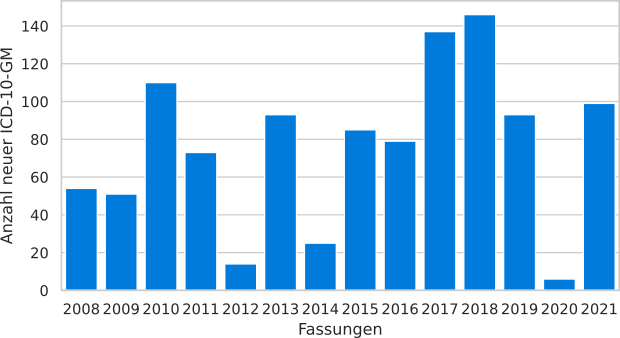
\includegraphics[height=7cm]{figures/newicdyear}
	\caption[Neue \acs{icd10gm} pro Jahr]{Anzahl neuer \acs{icd10gm} zwischen den Jahren 2008 und 2021}
	\label{fig:newicdyear}
\end{figure} 

Im Jahr 2018 wurden mehr als {\ttfamily 80} neue \ac{icd10gm} im Kapitel {\ttfamily Krankheiten des Muskel-Skelett-Systems und des Bindegewebes} eingefügt (Abbildung \ref{fig:newicdcap}). Ursache davon war die Insertion der Lokalisation der Muskel-Skelett-Beteiligung in der fünften Stelle der Kodierung mit Ziffern von {\ttfamily 0} bis {\ttfamily 9}, um die Beschreibung der Pathologien zu verbessern.

\begin{figure}[ht]
	\centering
	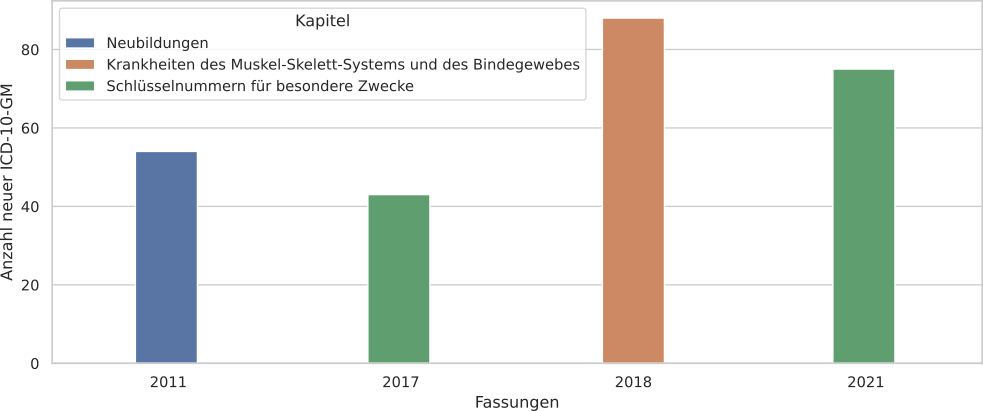
\includegraphics[height=7.5cm]{figures/kaptnrYear}
	\caption[Kapitel der \acs{icd10gm} pro Jahr]{Kapitel der neuen \acs{icd10gm} zwischen den Jahren 2008 und 2021}
	\label{fig:newicdcap}
\end{figure} 

Ein wichtiger und aktueller Punkt sind die meldepflichtigen Krankheiten in der Laufe der Jahre. Die Abbildung \ref{fig:newicdmeld} stellt das Verhältnis der meldepflichtigen \ac{icd10gm}. Es ist zu erkennen, dass sei 2007 nur in den Jahren 2010, 2016 und 2021 wurden neue meldepflichtigen Codes definiert (Tabelle \ref{tab:meldung}). Ursachen davon sind Pandemien und Epidemien wie die Influenza zwischen 2009 und 2010 \cite{influenza1, influenza2}, die Verbreitung des Dengue Fiebers in Europa als Effekt der Globalisierung mit der steigenden Mobilität \cite{denge1} und Verbreitung der asiatischen Tigermücke \textsl{Aedes (Stegomyia) albopictus} zwischen 2015 und 2016 in der Region als Konsequenz der milden Winter \cite{denge2}, und noch aktuell seit Februar 2020 die Verbreitung des Corona Virus in Europa \cite{corona1} und deren gesundheitlichen Folgen \cite{corona2}.

%\newpage
\begin{figure}[ht]
	\centering
	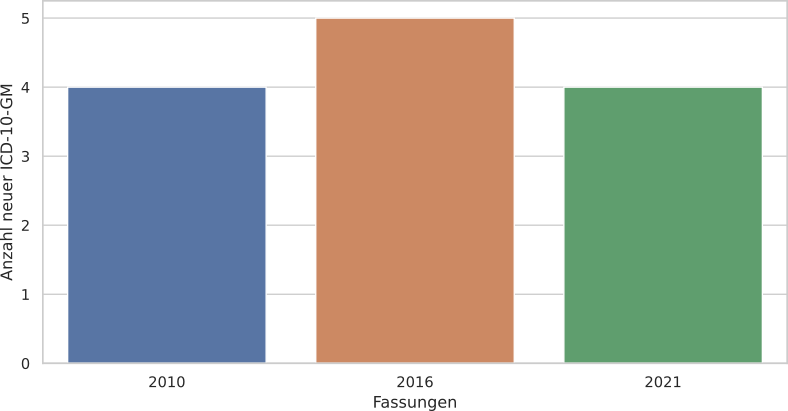
\includegraphics[height=5cm]{figures/arztJaYear}
	\caption[Meldepflichtige \acs{icd10gm} pro Jahr]{Meldepflichtige Krankheiten zwischen den Jahren 2008 und 2021}
	\label{fig:newicdmeld}
\end{figure} 

%\newpage
\begin{table}[ht]
	\centering
	\small
	\caption[Meldepflichtige \acs{icd10gm}]{Meldepflichtige Krankheiten}
	\label{tab:meldung}
	\begin{tabular}{|l|l|p{10.5cm}|}
		\hline
		\rowcolor{lightgray} Fassung & \acs{icd10gm} & Titel \\ \hline
		2010 & B17.9 & Akute Virushepatitis, nicht näher bezeichnet \\ \hline
		2010 & U69.2-! & Sekundäre Schlüsselnummern für besondere epidemiologische Zwecke \\ \hline
		2010 & U69.20! & Influenza A/H1N1 Pandemie 2009 [Schweinegrippe] \\ \hline
		2010 & U69.21! & Influenza A/H5N1 Epidemie [Vogelgrippe] \\ \hline
		2016 & A97.- & Dengue \\ \hline
		2016 & A97.0 & Dengue ohne Warnzeichen \\ \hline
		2016 & A97.1 & Dengue mit Warnzeichen \\ \hline
		2016 & A97.2 & Schweres Dengue \\ \hline
		2016 & A97.9 & Dengue, nicht näher bezeichnet \\ \hline
		2021 & U07.1! & COVID-19, Virus nachgewiesen \\ \hline
		2021 & U07.2! & COVID-19, Virus nicht nachgewiesen \\ \hline
		2021 & U10.- & Multisystemisches Entzündungssyndrom in Verbindung mit COVID-19 \\ \hline
		2021 & U10.9 & Multisystemisches Entzündungssyndrom in Verbindung mit COVID-19, nicht näher bezeichnet \\ \hline
	\end{tabular}
\end{table}

\newpage

\subsection{Modifizierte \acs{icd10gm}}

Die verschiedene Änderungen an den Metadaten sind in der Tabelle \ref{tab:icdupd} ausgelistet. Es ist zu erkennen, dass die meiste Änderungen in Bezug zur Mortalitätslisten entstanden sind. Die Ursache davon ist, dass der Inhalt solche Listen bei der meiste \ac{icd10gm} im Jahr 2008 definiert wurde. Andererseits sind die Änderungen an diesen Felder minimal bei \ac{icd10gm}, bei deren diese Listen schon definiert wurden. Die zahlreiche Modifikationen an der Klassentitel entstehen durch Vorläge zur Weiterentwicklung der Klassifikation. Ein Beispiel davon ist die Schlüsselnummer {\ttfamily E10.31} mit dem Titel \glqq{\ttfamily\textcolor{blue}{Primär insulinabhängiger} Diabetes mellitus [Typ-1-Diabetes] \textcolor{red}{mit} Augenkomplika-\\tionen: Als entgleist bezeichnet}\grqq{}. Dieser Titel wurde zu \glqq{\ttfamily\textcolor{blue}{Primär insulinab-\\hängiger} Diabetes mellitus [Typ-1-Diabetes]\textcolor{red}{: Mit }Augenkomplikationen:\\ Als entgleist bezeichnet}\grqq{} in 2009. Die Änderung wurde in diesem Jahr durchgeführt, da eine fünfte Stelle in der Klassifikationen von {\ttfamily E10}  bis {\ttfamily E14} eingefügt wurde \cite{diab09}. Der Titel dieser \ac{icd10gm} wurde nochmal in 2014 zu \glqq{\ttfamily Diabetes mellitus, Typ 1: Mit Augenkomplikationen: Als entgleist bezeichnet}\grqq{} geändert. In diesem Jahr wurden die Titel von der \ac{who} an die gebräuchliche Terminologie angepasst \cite{diab14}.

\newpage

\begin{table}[ht]
	\centering
	\caption[Änderungen in den Metadaten]{Liste der Metadaten und Anzahl an Änderungen}
	\label{tab:icdupd}
	\begin{tabular}{|l|p{12cm}|}
		\hline
		\rowcolor{lightgray} Änderungen & Metadaten \\ \hline
		6949 & \textbf{Bezug zur Mortalitätsliste 3} \\ \hline		
		5 & Bezug zur Mortalitätsliste 3 (davon definiert) \\ \hline
		6348 & \textbf{Bezug zur Mortalitätsliste 1} \\ \hline
		2 & Bezug zur Mortalitätsliste 1 (davon definiert) \\ \hline
		%1193 & Art des Fehlers bei Geschlechtsbezug \\ \hline
		1111 & Klassentitel \\ \hline
		308 & \textbf{Untere Altersgrenze} \\ \hline
		42 & Untere Altersgrenze (davon relevant) \\ \hline
		299 & \textbf{Bezug zur Morbiditätsliste} \\ \hline
		11 & Bezug zur Morbiditätsliste (davon definiert) \\ \hline
		% 286 & Alter Fehlertyp \\ \hline
		286 & \textbf{Obere Altersgrenze} \\ \hline
		19 & Obere Altersgrenze (davon relevant) \\ \hline
		162 & Auswahl der Laborausschlussziffer des \acp{ebm}  \\ \hline
		118 & Art der Vier- und Fünfsteller \\ \hline
		69 & \textbf{Bezug zur Mortalitätsliste 4} \\ \hline
		0 & Bezug zur Mortalitätsliste 4 (davon definiert) \\ \hline
		68 & Geschlechtsbezug \\ \hline
		64 & \textbf{Bezug zur Mortalitätsliste 2} \\ \hline
		2 & Bezug zur Mortalitätsliste 2 (davon definiert) \\ \hline
		44 & Erster Dreisteller der Gruppe \\ \hline		
		40 & Meldepflicht \\ \hline
		31 & Sehr seltene Krankheit in Mitteleuropa \\ \hline				
		6 & Belegte Nummer \\ \hline
		3 & Paragraph 295 \\ \hline			
		2 & Klassifikationsebene \\ \hline
	\end{tabular}
\end{table}

\newpage